\documentclass[border=6pt]{standalone}
\usepackage{tikz}
\usepackage{pgfplots}
\usepackage{amssymb}
\pgfplotsset{compat=1.18}
\usetikzlibrary{arrows.meta,positioning,calc,pgfplots.groupplots}
\definecolor{pesblue}{RGB}{0,45,98}
\definecolor{partial}{RGB}{176,106,0}
% ---------------------------------------------------------------------------
% fig_replacement_results -- the six replacement-scope results scored on
% 2026-09-27, each a point estimate with its 95% CI, one row per lane.
% Data: outputs/finish_pending_2026-09-27/<lane>/result.json (score, ci95).
%   Panel A: Wilson 95% intervals on k/n; errors, timeouts and ungraded
%     tasks are failures in n. E6 also shows the graded-only value
%     (90/704 = 12.78%) and the bound if all 108 unjudged tasks passed
%     (198/812 = 24.38%).
%   Panel B: E13 BALROG native progression (%), per environment with
%     percentile-bootstrap 95% CIs (B = 10000, seed 20260927), and the overall
%     BALROG-convention score (mean of the six environment means) 26.1%,
%     normal-approximation CI [22.64, 29.56].
% Lanes are different suites with different metrics; no cross-lane average
% is drawn.
% ---------------------------------------------------------------------------
\begin{document}
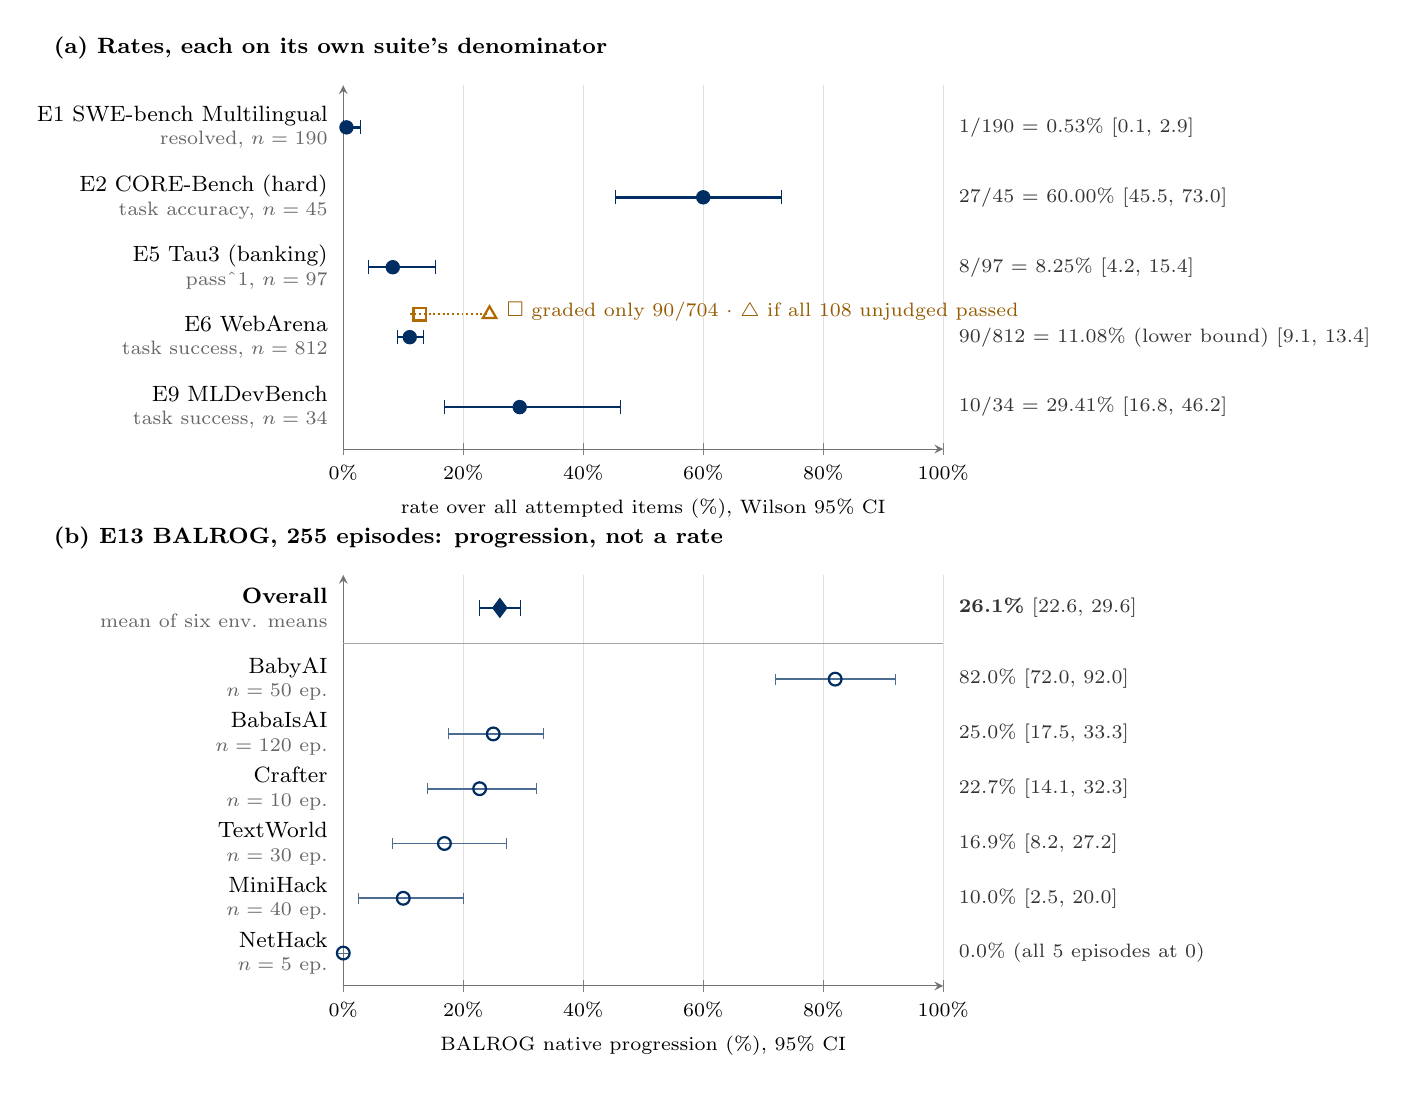
\begin{tikzpicture}[val/.style={anchor=west, font=\scriptsize, text=black!80}]
\begin{groupplot}[
  group style={group size=1 by 2, vertical sep=16mm},
  width=9.2cm, xmin=0, xmax=100,
  xtick={0,20,40,60,80,100}, xticklabel={\pgfmathprintnumber{\tick}\%},
  xmajorgrids, grid style={black!12},
  axis lines=left, axis line style={black!55},
  tick label style={font=\scriptsize},
  y tick label style={align=right, font=\footnotesize},
  ytick style={draw=none},
  clip=false,
]
\nextgroupplot[
  height=6.2cm, ymin=0.4, ymax=5.6,
  ytick={5,4,3,2,1},
  yticklabels={{E1 SWE-bench Multilingual\\[-1pt]{\color{black!60}\scriptsize resolved, $n=190$}},{E2 CORE-Bench (hard)\\[-1pt]{\color{black!60}\scriptsize task accuracy, $n=45$}},{E5 Tau3 (banking)\\[-1pt]{\color{black!60}\scriptsize pass\textasciicircum 1, $n=97$}},{E6 WebArena\\[-1pt]{\color{black!60}\scriptsize task success, $n=812$}},{E9 MLDevBench\\[-1pt]{\color{black!60}\scriptsize task success, $n=34$}}},
  xlabel={\scriptsize rate over all attempted items (\%), Wilson 95\% CI},
  title={\footnotesize\bfseries (a) Rates, each on its own suite's denominator},
  title style={at={(0,1)}, anchor=south west, xshift=-38mm},
]
\addplot[only marks, mark=*, mark size=2.4pt, color=pesblue,
  error bars/.cd, x dir=both, x explicit, error bar style={line width=0.9pt, color=pesblue},
  error mark options={rotate=90, mark size=2.5pt, color=pesblue}]
  coordinates {
  (0.53,5) += (2.39,0) -= (0.44,0)
  (60.0,4) += (12.98,0) -= (14.55,0)
  (8.25,3) += (7.19,0) -= (4.01,0)
  (11.08,2) += (2.35,0) -= (1.97,0)
  (29.41,1) += (16.76,0) -= (12.58,0)
  };
% E6 sensitivity markers (not estimates of a different quantity; bounds on the same one)
\addplot[only marks, mark=square, mark size=2.3pt, line width=0.8pt, color=partial]
  coordinates {(12.78,2.33)};
\addplot[only marks, mark=triangle, mark size=2.8pt, line width=0.8pt, color=partial]
  coordinates {(24.38,2.33)};
\draw[partial, densely dotted, line width=0.7pt] (axis cs:11.08,2.33) -- (axis cs:24.38,2.33);
\node[font=\scriptsize, color=partial!85!black, anchor=west] at (axis cs:25.6,2.36)
  {$\square$ graded only 90/704 $\cdot$ $\triangle$ if all 108 unjudged passed};
\node[val] at (axis cs:101,5) {$1/190$ $=$ 0.53\% [0.1, 2.9]};
\node[val] at (axis cs:101,4) {$27/45$ $=$ 60.00\% [45.5, 73.0]};
\node[val] at (axis cs:101,3) {$8/97$ $=$ 8.25\% [4.2, 15.4]};
\node[val] at (axis cs:101,2) {$90/812$ $=$ 11.08\% (lower bound) [9.1, 13.4]};
\node[val] at (axis cs:101,1) {$10/34$ $=$ 29.41\% [16.8, 46.2]};
\nextgroupplot[
  height=6.8cm, ymin=0.4, ymax=7.9,
  ytick={6,5,4,3,2,1,7.3},
  yticklabels={{BabyAI\\[-1pt]{\color{black!60}\scriptsize $n=50$ ep.}},{BabaIsAI\\[-1pt]{\color{black!60}\scriptsize $n=120$ ep.}},{Crafter\\[-1pt]{\color{black!60}\scriptsize $n=10$ ep.}},{TextWorld\\[-1pt]{\color{black!60}\scriptsize $n=30$ ep.}},{MiniHack\\[-1pt]{\color{black!60}\scriptsize $n=40$ ep.}},{NetHack\\[-1pt]{\color{black!60}\scriptsize $n=5$ ep.}},{\textbf{Overall}\\[-1pt]{\color{black!60}\scriptsize mean of six env. means}}},
  xlabel={\scriptsize BALROG native progression (\%), 95\% CI},
  title={\footnotesize\bfseries (b) E13 BALROG, 255 episodes: progression, not a rate},
  title style={at={(0,1)}, anchor=south west, xshift=-38mm},
]
\draw[black!35] (axis cs:0,6.65) -- (axis cs:100,6.65);
\addplot[only marks, mark=o, mark size=2.3pt, line width=0.8pt, color=pesblue,
  error bars/.cd, x dir=both, x explicit, error bar style={line width=0.7pt, color=pesblue!70},
  error mark options={rotate=90, mark size=2pt, color=pesblue!70}]
  coordinates {
  (82.0,6) += (10.00,0) -= (10.00,0)
  (25.0,5) += (8.33,0) -= (7.50,0)
  (22.73,4) += (9.54,0) -= (8.64,0)
  (16.86,3) += (10.39,0) -= (8.62,0)
  (10.0,2) += (10.00,0) -= (7.50,0)
  (0.0,1) += (0.00,0) -= (0.00,0)
  };
\addplot[only marks, mark=diamond*, mark size=3.4pt, color=pesblue,
  error bars/.cd, x dir=both, x explicit, error bar style={line width=1.0pt, color=pesblue},
  error mark options={rotate=90, mark size=2.8pt, color=pesblue}]
  coordinates {(26.10,7.3) += (3.46,0) -= (3.46,0)};
\node[val] at (axis cs:101,7.3) {\textbf{26.1\%} [22.6, 29.6]};
\node[val] at (axis cs:101,6) {82.0\% [72.0, 92.0]};
\node[val] at (axis cs:101,5) {25.0\% [17.5, 33.3]};
\node[val] at (axis cs:101,4) {22.7\% [14.1, 32.3]};
\node[val] at (axis cs:101,3) {16.9\% [8.2, 27.2]};
\node[val] at (axis cs:101,2) {10.0\% [2.5, 20.0]};
\node[val] at (axis cs:101,1) {0.0\% (all 5 episodes at 0)};
\end{groupplot}
\end{tikzpicture}
\end{document}
